%!TEX root = ../main.tex
\begin{example}[Salary Update Error]\label{ex:telco}
  A manager updates the tax amount with $30\%$ tax rate for high income employees that earn more than $\$87500$.
  She submits this through a form in the salary accounting application, 
  but due to keyboard slip, incorrectly types $\$85700$ for the income threshold.  
  Later queries that insert new paychecks, compute tax calculations,
  aggregate department salaries end up propogating this error throughout other records in the database, leading to
  employee dissatifaction.  Figure~\ref{fig:example} illustrates a concrete example where $Q_1$, $Q_2$, and $Q_3$ are executed on an 
  initial salary database $D_0$.  The error in $Q_1$ that incorrectly sets some of the tax rates is propogated to other fields in the table.
\end{example}

\begin{figure}[t]
    \centering
        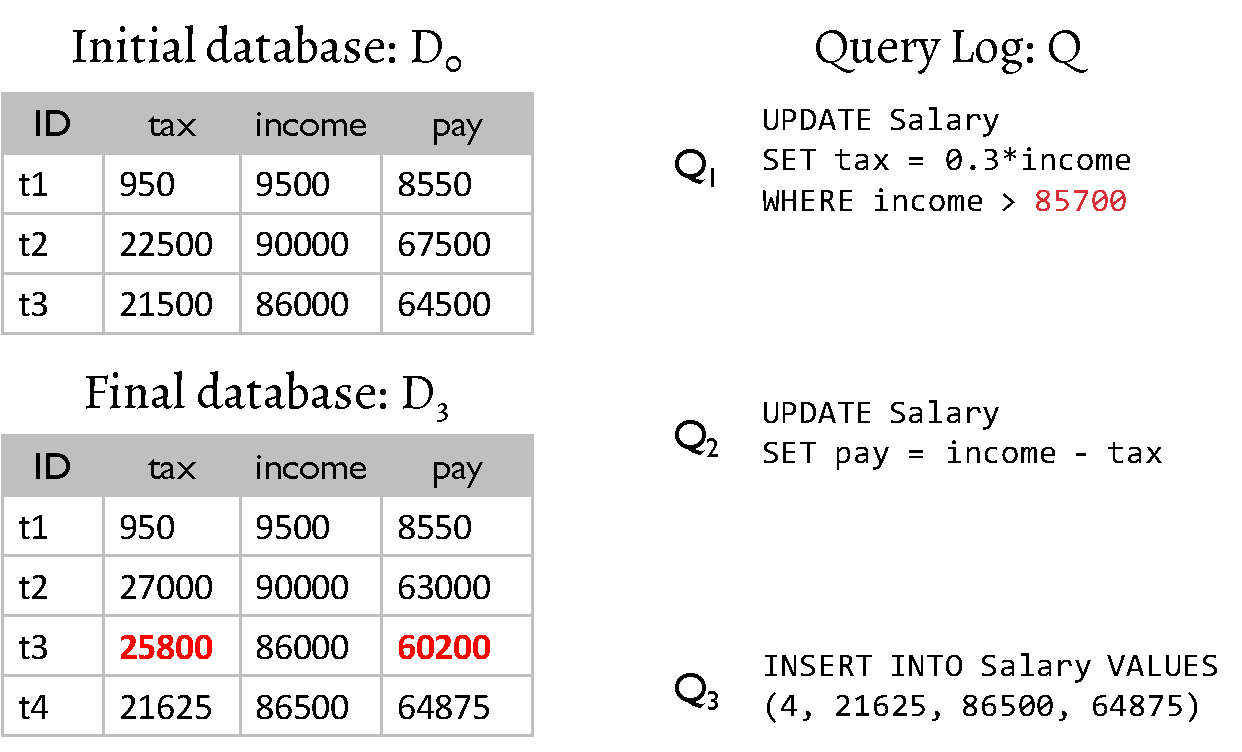
\includegraphics[width=0.45\textwidth]{figures/example2}
    \caption{$Q_1$ updates the tax amount with $30\%$ tax rate 
      for high income employees using an incorrect predicate.  
      The error is propogated by $Q_2$ to the $pay$ field in the database.
      Finally, a benign insert query $Q_3$ inserts correct salary information. 
      The final database state contains a mixture of incorrect and correct salary data.
    }
    \label{fig:example}
\end{figure}


In this example, by the time errors in the database have been detected, 
perhaps by employees that report their encorrect paystubs, it is difficult 
to both identify all of the other errors in the database, and to trace these errors back to the erroneous query to correct it.
This example can occur in any data processing systems where manual input is used to generate queries that modify the database --
this could be in the form of adhoc queries executed by a system administrator, or web-based forms that construct queries based
on user input, or even stored procedures that use human input to fill the parameter values.
